\chapter{A case study: spawn points placement}

% INTRODUCTION %

In this chapter we discuss a case study we designed to test the effectiveness of our framework. We
performed an experiment with real users to validate the placement heuristics for spawn points and, at the same time, to test the data-collection capabilities of our framework, that was used to setup and manage the experiment.

% DESCRIPTION %

\section{Goals}

We designed this experiment to analyze how our methods for the placement of spawn points influence the up-player vs down-player dynamic and to prove their effectiveness. We tried to recreate the situation where the up-player, once killed his opponent, tries to find him as soon as possible, just after his respawn, to score another easy kill. As we have seen, a well-designed map should slow down this operation by having its spawn points in areas that are not central, are easy to leave and covered. In this experiment we compared two approaches: the \<uniform> one, that selects rooms with the uniform method (see chapter \ref{sss:room_selection}) and tiles with the heuristic defined for spawn points, and the \<heuristic> one, that selects both rooms and tiles with the heuristics defined for spawn points (see chapter \ref{sss:sph}) and should allow to obtain a placement of spawn point coherent with the one described above. These two approaches use the same method to select tiles to focus on the effects of room selection, since the ones of tile selection are rather obvious (an object on a tile with a low visibility is difficult to find).

\par

To highlight this gameplay dynamic, we designed a game mode where the user, which represents the up-player, must find and destroy a static target, which represents the down-player, as many times as possible before times runs out. Each time that the user destroys a target, it respawns at a random spawn point. The user cannot die and has infinite ammunition, so he does not have to look for resources.

% SETUP %

\section{Experimental design}

For this experiment, we setup the \<Experiment Manager> to propose in each play session a quick tutorial, two matches and a survey. The experiment was composed by three \<studies>, corresponding to three different maps, each one composed by two \<cases>, one corresponding to the map populated with the heuristic approach and one corresponding to a pool of five versions of the map populated with the uniform approach\footnote{When selecting rooms with the uniform method the first one is chosen at random. This allows to obtain multiple versions of the same map.}. In a play session, the user played the same map twice, once with the heuristic distribution and once with the uniform distribution, in a random order and with the map flipped in one of the two matches. We used the survey to profile each user according to their skill and familiarity with video games and FPS and to get a feedback about the match in which they found it harder to locate the targets. The experiment was deployed online and played by the users via browser on their own computers.

\par

As game mode, we used \<Target Hunt>, with the game duration set to three minutes, the list of spawnable entities composed of just one target and an \<assault rifle> with infinite ammunition as the only weapon available to the player. The maps were stored as text files and were loaded by the \<Divisive Generator> and displayed with the \<Prefab Assembler>. 

\par

For each match, a complete game log was saved, along with the following performance metrics, saved in a separate log:
\begin{itemize}
\item \<TargetLogs>: this field contains a list of all the targets that the user managed to destroy. Each entry contains a timestamp, the coordinates of the destroyed target, the coordinates of the user, the distance covered by the user and the time passed during the lifespan of the target.
\item \<Shots>: the total number of projectiles shot by the user.
\item \<Hits>: the number of projectiles that hit a target.
\item \<Accuracy>: the percentage of projectiles that hit a target.
\item \<Kills>: the total number of targets destroyed by the user.
\item \<Distance>: the total distance covered by the user during the match, considering his complete trajectory and cells of unitary width as reference unit.
\item \<AvgKillTime>: the average time needed by the user to find a target, computed as the duration of the match divided by the number of kills.
\item \<AvgKillDistance>: the average distance covered by the user to find a target, computed as \<Distance> divided by the number of kills.
\end{itemize}

\noindent
The performance of the player is measured by \<AvgKillTime> and \<AvgKillDistance>, that are also indicators of how difficult it is to find targets in the map. The answers to the survey were saved as well.

\par

The three maps that we have selected for this experiment have very different layouts:

\begin{itemize}
\item \<Arena>: this map presents a wide arena, two sides of which are adjacent to parallel corridors with many openings. As the visibility heatmap in figure \ref{img:arena_visibility} shows, the central arena allows to control most of the map, whereas the corridors offer some repair and perfect spots to place spawn points. Figure \ref{img:arena_safe} shows the spawn points positioned using the heuristic approach, whereas figure \ref{img:arena_uniform} shows one of the five configuration produced with the uniform approach.
\item \<Corridors>: this map presents many small rooms connected by long corridors. As it can be seen in figure \ref{img:corridors_visibility}, there is no area that allows to control the others and the only points with high visibility are the ones where corridors intersect. Figure \ref{img:corridors_safe} shows the spawn points positioned using the heuristic approach, whereas figure \ref{img:corridors_uniform} shows one of the five configuration produced using the uniform approach.
\item \<Intense>: compared to the previous two, this map presents an intermediate layout, since it has both open areas and small rooms connected by corridors. As it can be seen in figure \ref{img:intense_visibility}, this reflects also on the visibility, that is high in the open areas and low in the remaining sections of the map. Figure \ref{img:intense_safe} shows the spawn points positioned using the heuristic approach, whereas figure \ref{img:intense_uniform} shows one of the five configuration produced using the uniform approach.
\end{itemize}

\begin{figure}[p]
\centering
\begin{subfigure}[t]{0.3\linewidth}
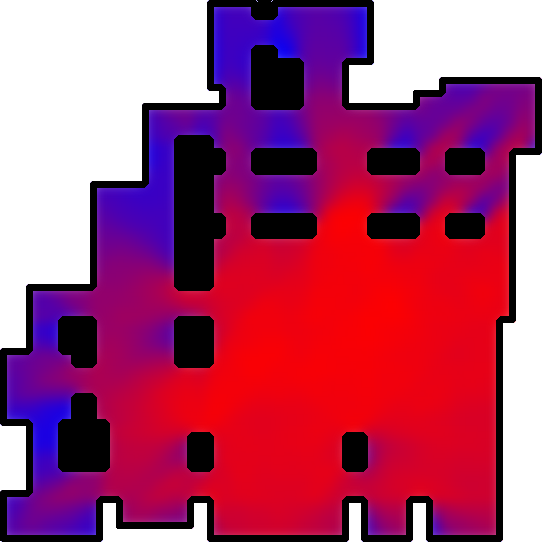
\includegraphics[width=\linewidth]{arena_visibility}
\caption{Heatmap showing the visibility of the level.}
\label{img:arena_visibility}
\end{subfigure} 
\hfil
\begin{subfigure}[t]{0.3\linewidth}
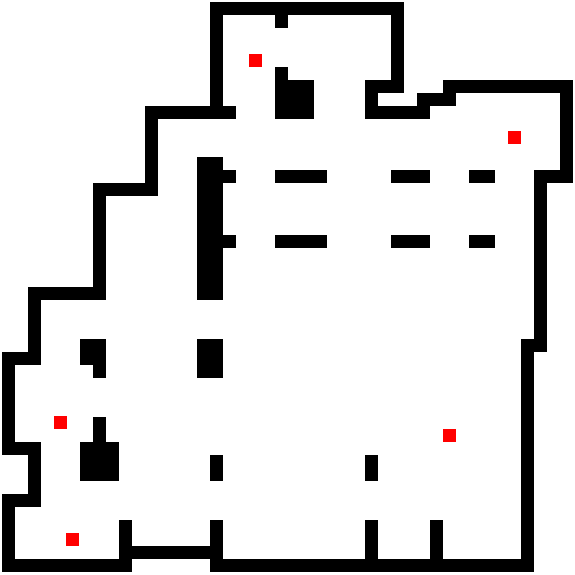
\includegraphics[width=\linewidth]{arena_safe}
\caption{Spawn points (in red) placed using the heuristic approach.}
\label{img:arena_safe}
\end{subfigure}
\hfil
\begin{subfigure}[t]{0.3\linewidth}
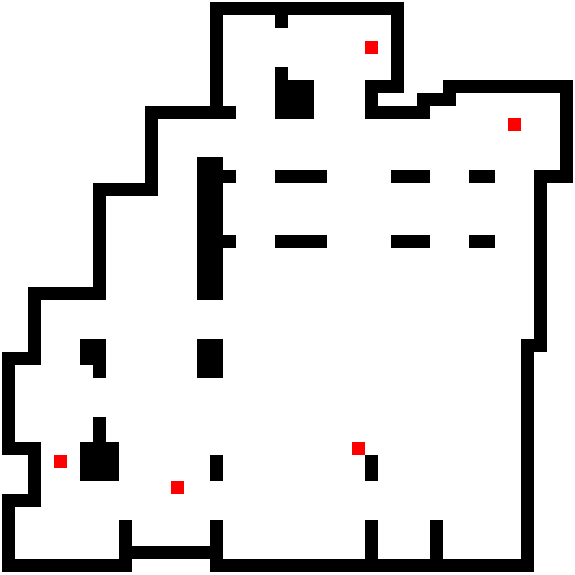
\includegraphics[width=\linewidth]{arena_uniform}
\caption{Spawn points (in red) placed using the uniform approach.}
\label{img:arena_uniform}
\end{subfigure} 
\caption{``Arena'' map used in the experiment.}
\label{img:arena}
\vspace{0.4cm}
\begin{subfigure}[t]{0.3\linewidth}
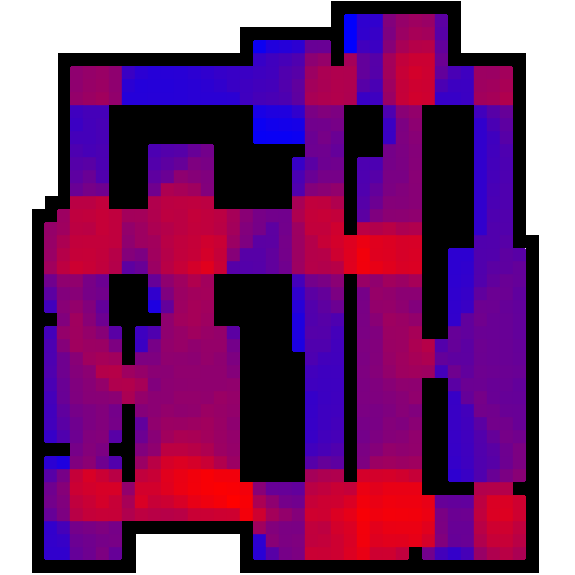
\includegraphics[width=\linewidth]{corridors_visibility}
\caption{Heatmap showing the visibility of the level.}
\label{img:corridors_visibility}
\end{subfigure} 
\hfil
\begin{subfigure}[t]{0.3\linewidth}
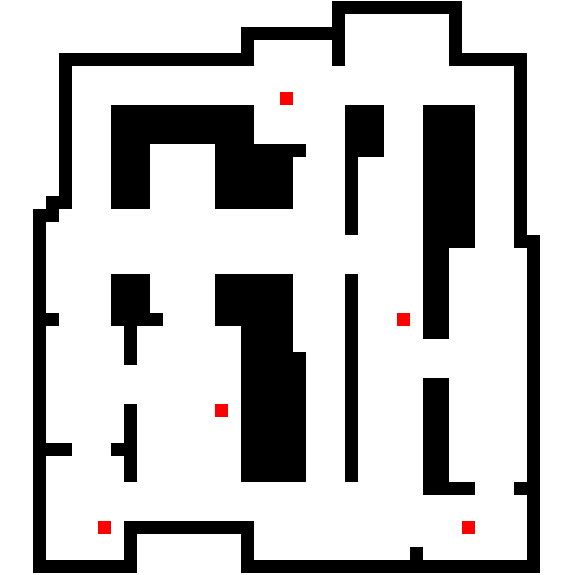
\includegraphics[width=\linewidth]{corridors_safe}
\caption{Spawn points (in red) placed using the heuristic approach.}
\label{img:corridors_safe}
\end{subfigure}
\hfil
\begin{subfigure}[t]{0.3\linewidth}
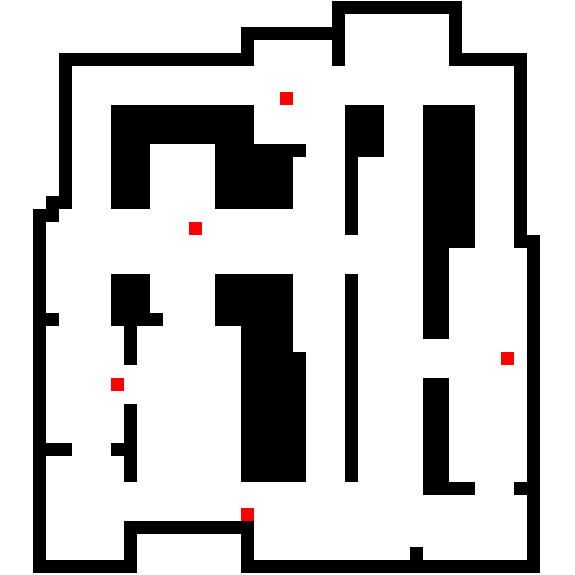
\includegraphics[width=\linewidth]{corridors_uniform}
\caption{Spawn points (in red) placed using the uniform approach.}
\label{img:corridors_uniform}
\end{subfigure} 
\caption{``Corridors'' map used in the experiment.}
\label{img:corridors}
\vspace{0.4cm}
\begin{subfigure}[t]{0.3\linewidth}
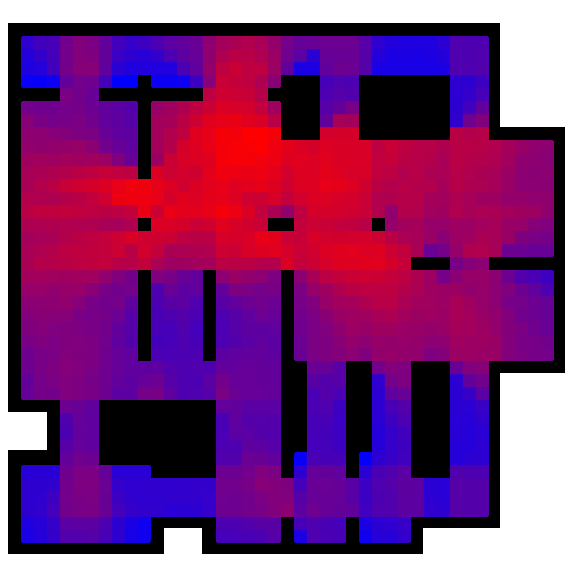
\includegraphics[width=\linewidth]{intense_visibility}
\caption{Heatmap showing the visibility of the level.}
\label{img:intense_visibility}
\end{subfigure} 
\hfil
\begin{subfigure}[t]{0.3\linewidth}
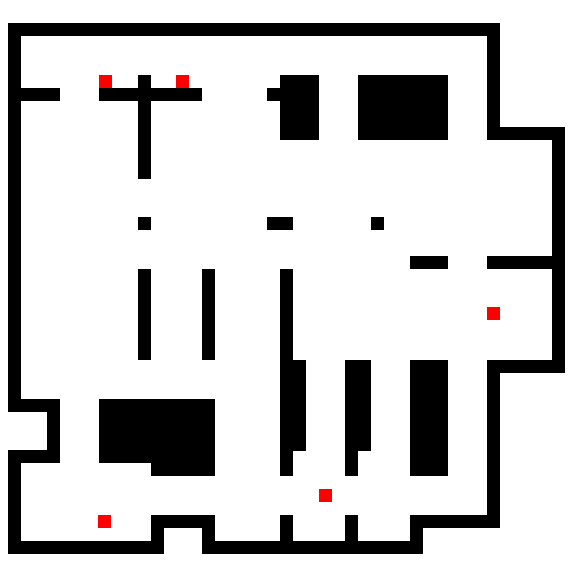
\includegraphics[width=\linewidth]{intense_safe}
\caption{Spawn points (in red) placed using the heuristic approach.}
\label{img:intense_safe}
\end{subfigure}
\hfil
\begin{subfigure}[t]{0.3\linewidth}
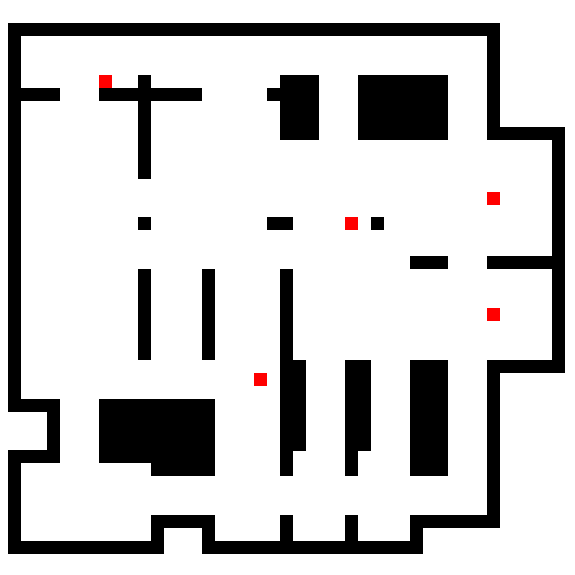
\includegraphics[width=\linewidth]{intense_uniform}
\caption{Spawn points (in red) placed using the uniform approach.}
\label{img:intense_uniform}
\end{subfigure}
\caption{``Intense'' map used in the experiment.}
\label{img:intense} 
\end{figure}

As we have said, the heuristic and the uniform approaches select rooms with two different criteria, but they employ the same logic when selecting tiles. This means that the two heuristics select tiles which have similar visibility conditions, so the player's performance depends exclusively on how the rooms have been selected. This is observable in figures \ref{img:arena}, \ref{img:corridors} and \ref{img:intense}: when the uniform approach happens to select a room that has been selected also by the heuristic one, the spawn point is placed exactly on the same tile.

% RESULTS %

\section{Results}

\begin{table}
\setlength\extrarowheight{2pt}
\begin{tabularx}{\textwidth}{|l|C|C|C|C|C|}
\cline{3-6}
\multicolumn{2}{c|}{} & Total & Arena & Corridors & Intense \\
\hline
\multicolumn{2}{|l|}{Number of samples} & 27 & 10 & 9 & 8 \\
\hline
\multirow{ 2}{*}{$\mu(\text{Shots})$} & Heuristic & 104.04 & 114.89 & 101.00 & 94.88 \\
\cline{2-6}
& Uniform & 117.44 & 131.33 & 100.25 & 119.00 \\
\hline
\multirow{ 2}{*}{$\mu(\text{Hits})$} & Heuristic & 42.68 & 48.44 & 43.50 & 35.38 \\
\cline{2-6}
& Uniform & 50.12 & 54.22 & 44.50 & 51.13 \\
\hline
\multirow{ 2}{*}{$\mu(\text{Accuracy})$} & Heuristic & 0.45 & 0.43 & 0.51 & 0.40 \\
\cline{2-6}
& Uniform & 0.48 & 0.45 & 0.52 & 0.48 \\
\hline
\multirow{ 2}{*}{$\mu(\text{Kills})$} & Heuristic & 10.06 & 10.75 & 10.44 & 8.75 \\
\cline{2-6}
& Uniform & 11.88 & 12.27 & 10.67 & 12.75 \\
\hline
\multirow{ 2}{*}{$\mu(\text{Distance})$} & Heuristic & 675.22 & 633.56 & 675.43 & 716.68 \\
\cline{2-6}
& Uniform & 680.79 & 649.62 & 688.34 & 704.42 \\
\hline
\multirow{ 2}{*}{$\mu(\text{AvgKillTime})$} & Heuristic & 20.24 & 21.09 & 18.25 & 21.40  \\
\cline{2-6}
& Uniform & 16.06 & 15.50 & 17.46 & 15.18 \\
\hline
\multirow{ 2}{*}{$\mu(\text{AvgKillDistance})$} & Heuristic & 73.34 & 64.21 & 70.90 & 84.90 \\
\cline{2-6}
& Uniform & 60.70 & 55.24 & 68.13 & 58.72 \\
\hline
\multirow{ 2}{*}{$\mode(\text{Difficulty})$} & Effective & heuristic & heuristic & uniform & heuristic \\
\cline{2-6}
& Percived & heuristic & heuristic & equal & heuristic \\
\hline
\end{tabularx}
\caption[The information retrieved from the dataset.]{The information retrieved from the dataset. $\mu$ denotes the mean value and $\mode$ denotes the modal value.}
\label{tab:means}
\end{table}

The data collected with this experiment consisted of 27 samples. As table \ref{tab:means} shows, of these 27 samples, 10 are pairs of matches played in map ``Arena'', 9 are pairs of matches played in map ``Corridors'' and 8 are pairs of matches played in map ``Intense''. The table also shows the values of the metrics that we have defined divided by map and placement method.

\par

As we have seen, the performance of the player is measured with \<AvgKillTime> and \<AvgKillDistance> and by computing their mean values we observed that the users performed better in the matches associated to the uniform approach with respect to the ones associated to heuristic approach. For the former the mean value of \<AvgKillTime> is $16.06$ seconds and the one of \<AvgKillDistance> is $60.7$ cells, whereas for the latter the mean value of \<AvgKillTime> is $20.24$ seconds and the one of \<AvgKillDistance> is $73.34$ cells. The respective increase of $26\%$ and $21\%$ on the average time and distance needed to find a target confirms that spawn points placed with the heuristic approach are more difficult to find than the ones placed with the uniform approach.

\par

To test the statistical significance of this result, we performed the \<Wilcoxon> statistical test\footnote{The \<Wilcoxon signed-rank test> is a \<non-parametric statistical hypothesis test> used to compare two matched samples to assess whether their population mean ranks differ.} by \<Pratt>\footnote{With respect to the standard Wilcoxon test, the one by Pratt considers also the observations for which the difference of the elements in the pair is zero. We opted for this approach since some samples happen to have metrics with the same value for the two placements.}, using as matched samples the values assumed by the metric at issue when using heuristic placement and when using uniform placement. Both \<AvgKillTime> and  \<AvgKillDistance> passed the test, the former with $\alpha = 0.00203 < 0.005$, one-tiled, and the latter with $\alpha = 0.01243 < 0.05$, one-tiled.

\begin{figure}
\centering
\begin{subfigure}[t]{0.49\linewidth}
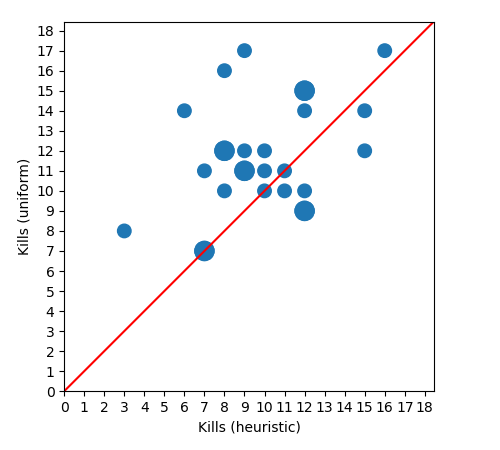
\includegraphics[width=\linewidth]{scatter_kills}
\caption{Kills.}
\label{img:scatter_kills}
\end{subfigure}
\hfill
\begin{subfigure}[t]{0.49\linewidth}
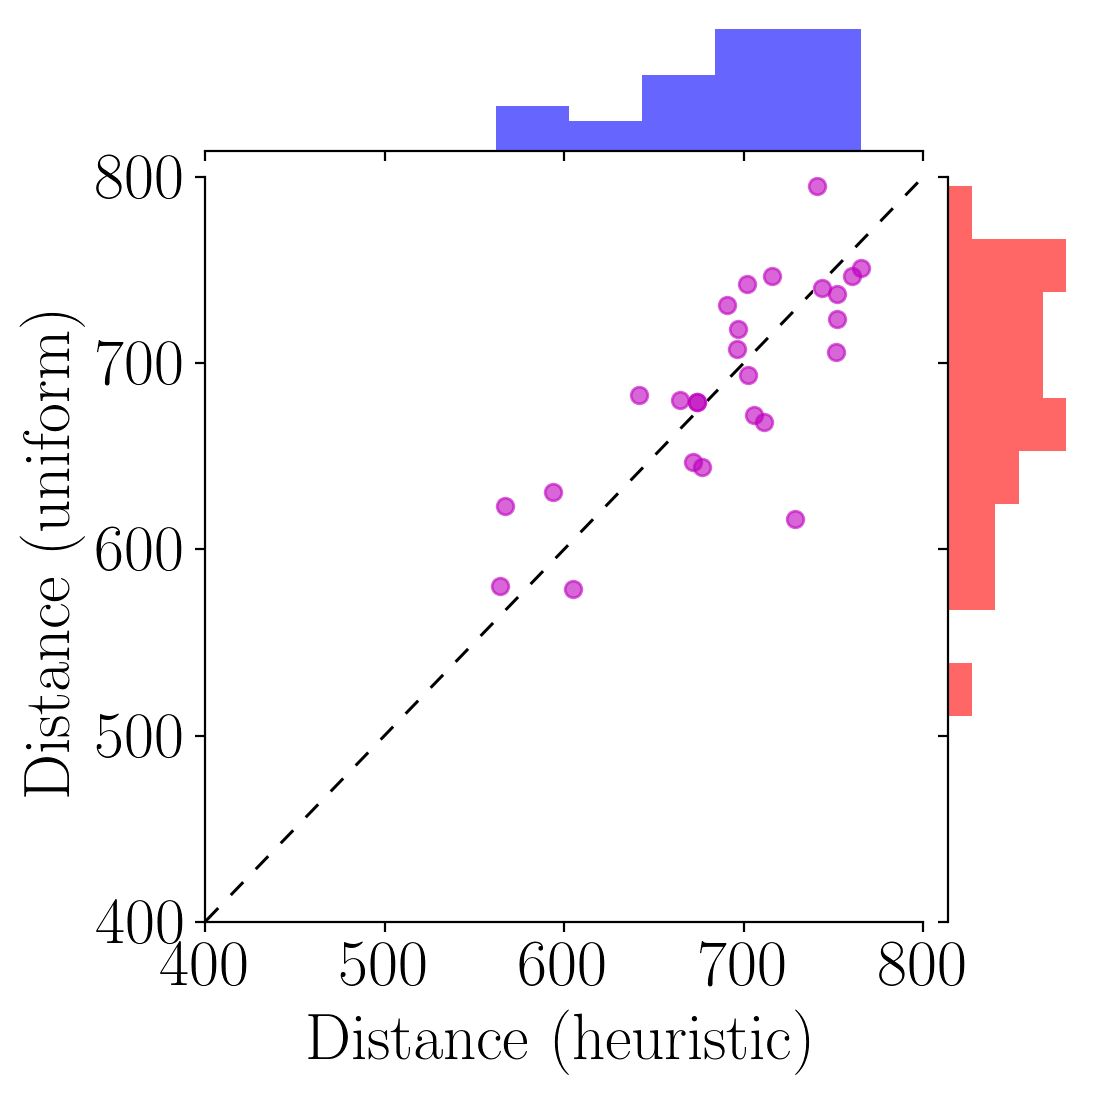
\includegraphics[width=\linewidth]{scatter_distance}
\caption{Distance.}
\label{img:scatter_distance}
\end{subfigure}

\begin{subfigure}[t]{0.49\linewidth}
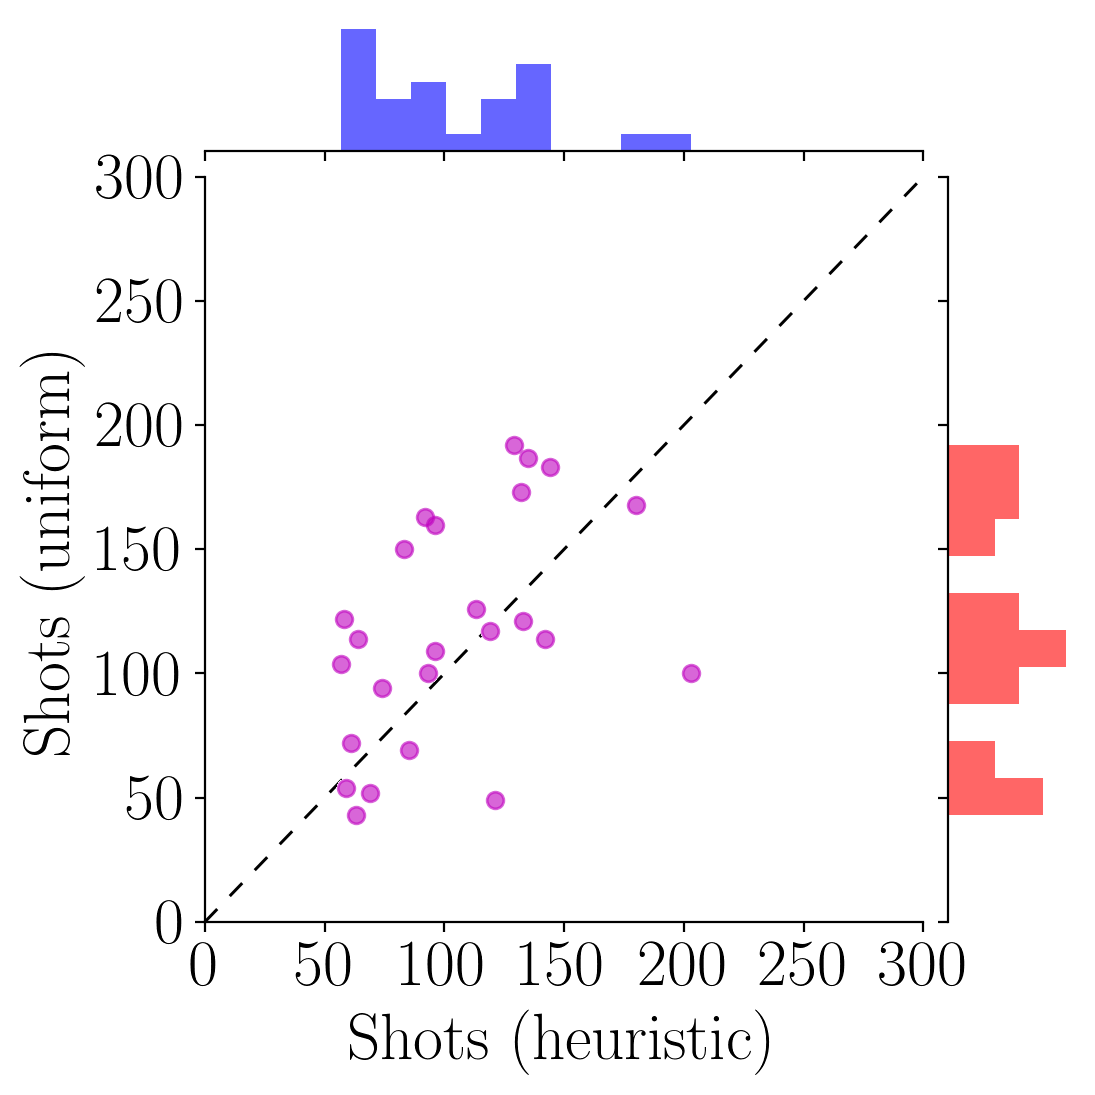
\includegraphics[width=\linewidth]{scatter_shots}
\caption{Shots.}
\label{img:scatter_shots}
\end{subfigure}
\hfill
\begin{subfigure}[t]{0.49\linewidth}
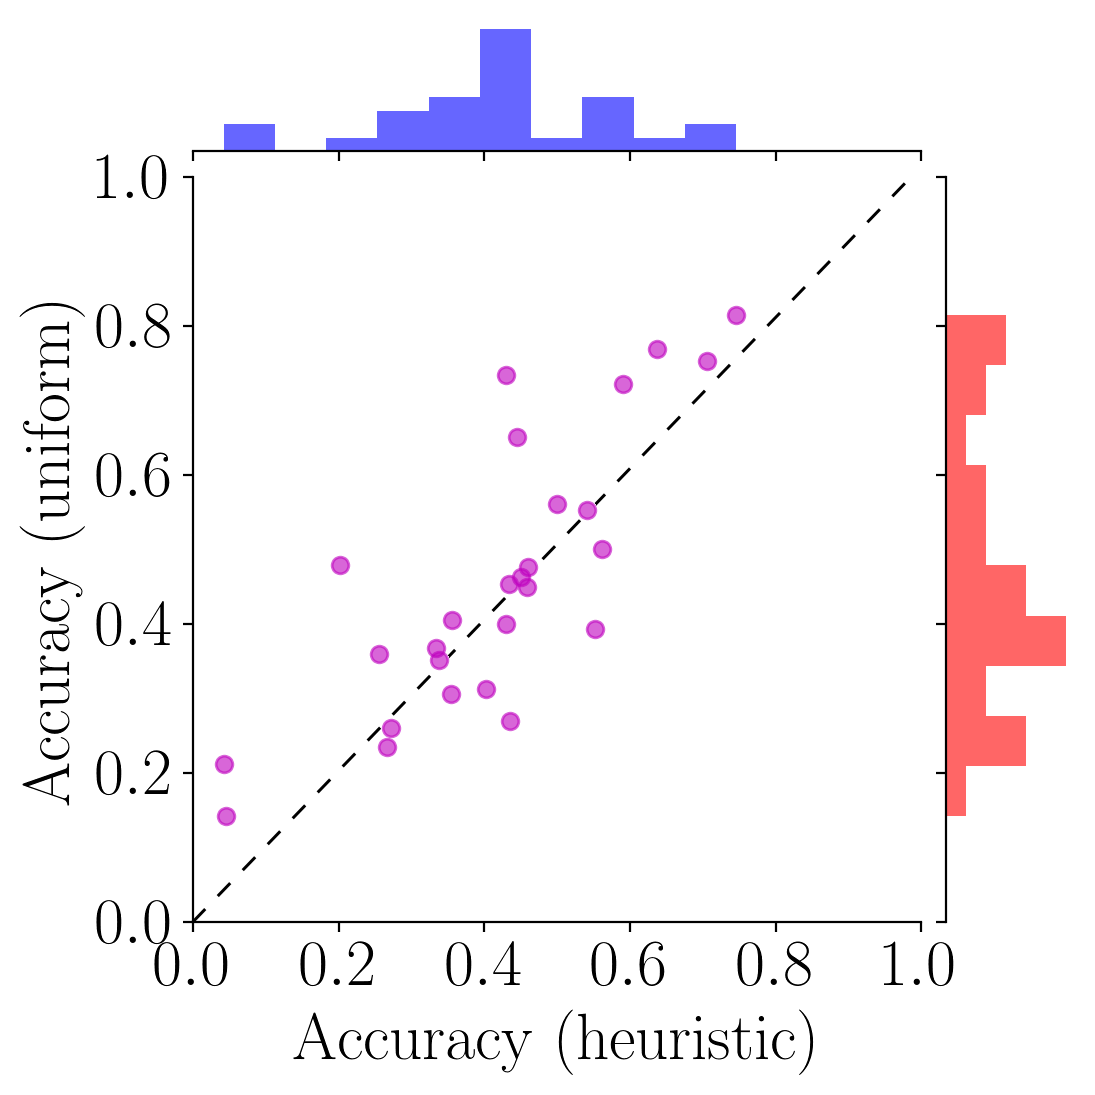
\includegraphics[width=\linewidth]{scatter_accuracy}
\caption{Accuracy.}
\label{img:scatter_accuracy}
\end{subfigure}
\caption[Experiment outcomes by metrics.]{Experiment outcomes by metrics. The outcome associated to the heuristic approach is on the horizontal axis, the one associated to the uniform approach is on the vertical axis.}
\label{img:metrics} 
\end{figure}

The effect of the two approaches on the metrics can also be analyzed by plotting their values, assigning to the horizontal axis the value of the metric in maps with heuristic placement and to the vertical axis the value of the metric in maps with uniform placement. Each point of such graph represents the outcome of a test whose coordinates are the values of the metric in the two matches. By tracing the bisector, it is easy to see for which of the two approaches a metric is higher. If the points are scattered under the bisector it means that the metric tends to be higher for the heuristic approach, whereas if they are scattered above the bisector it means that the metric tends to be higher for the uniform approach. Figure \ref{img:metrics} shows such graphic for each metric:

\begin{itemize}
\item \<Kills>: as figure \ref{img:scatter_kills} shows, the number of kills tends to be higher with the uniform placement ($11.88 > 10.06$, considering the mean values). This result is rather obvious, since, as we have seen analyzing \<AvgKillTime> and \<AvgKillDistance>, targets are more difficult to find with the heuristic placement. The Wilcoxon test, which is passed with $\alpha = 0.00347 < 0.005$, one-tiled, confirms this outcome. 
\item \<Distance>: as figure \ref{img:scatter_distance} shows, the total distance covered by users is not influenced by the employed placement method ($680.79\approx675.22$, considering the mean values). This is due to the fact that users are constantly moving and the agility with which they navigate the map depends exclusively on their familiarity with FPS games and on the layout of the map. The Wilcoxon test, which is not passed with $\alpha = 0.294 > 0.05$, one-tiled, confirms this outcome.
\item \<Shots>: as figure \ref{img:scatter_shots} shows, the number of shots tends to be higher with the uniform placement ($117.44 >  104.04$, considering the mean values). This result is coherent with what we have observed for \<Kills>, to which \<Shots> is expected to be directly proportional. The Wilcoxon test, which is passed with $\alpha = 0.0336 < 0.05$, one-tiled, confirms this outcome.
\item \<Accuracy>: as figure \ref{img:scatter_accuracy} shows, the accuracy is not significantly influenced by the used placement method ($45\% \approx 48\%$, considering the mean values). This is due to the fact that the accuracy depends almost exclusively on the aiming skills of the user. The Wilcoxon test, which is not passed with $\alpha = 0.294 > 0.05$, one-tiled, confirms this outcome.
\end{itemize}

We also observed that the effects of the placement were considerably different depending on the layout of the map. With the heuristic placement, map ``Arena'' had a mean number of kills of $10.75$, map ``Corridors'' of $10.44$ and map ``Intense'' of $8.75$. We expected the one of ``Arena'' to be the highest, because of its central area that dominates the rest of the map, but we did not expect the ones of ``Corridors'' to be almost as high, since its structure is more difficult to navigate. Moreover, we expected an intermediate number of kills in ``Intense'', since it merges the features of the two other maps, but it proved to be the map where targets were harder to find. This could be explained by the fact that ``Corridors'', even if more complex than ``Arena'', has a rather regular structure and its long corridors allow to easily spot a target. Instead, for what concerns ``Intense'', its structure is rather complex and difficult to navigate and since the central open area does not allow to control all of the map the tactical advantage it provides is not so strong. With the uniform placement the mean number of kills of ``Arena'' increased to $11.88$, the one of ``Corridors'' remained almost the same ($10.67$) and the one of ``Intense'' increased dramatically to $12.75$. The reasons for such different reactions lies in the layout of each map. The central area of ``Arena'' allows to control all of the surroundings, so the placement of spawn points in areas that are less visible has a relevant effect. ``Corridors'', instead, has a regular structure and the number of intersections between its corridors is almost always the same, so it is not relevant where spawn points are placed, since all the rooms have the same features. Finally, the tangled structure of ``Intense'' offers to the heuristic approach a lot of interesting spots where to place spawn points and the presence of an area that allows a partial control of the map makes this choice even more meaningful. This shows that the effects of the heuristic approach are more pronounced in maps which layout is not uniform.

\begin{figure}
	\centering
	\hfill
  	\begin{subfigure}[t]{0.385\linewidth}
		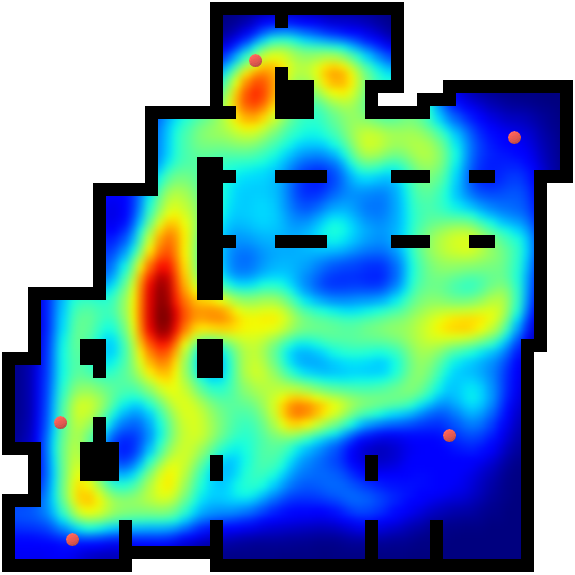
\includegraphics[width=\linewidth]{heat_arena_safe}
     		\caption{Map ``Arena'' with heuristic placement.}
     		\label{img:heat_arena_safe}
 	\end{subfigure}
 	\hfill
  	\begin{subfigure}[t]{0.385\linewidth}
    		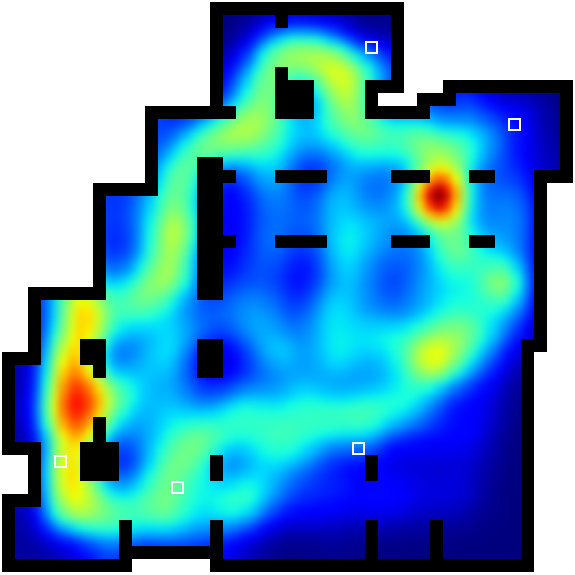
\includegraphics[width=\linewidth]{heat_arena_uniform}
     		\caption{Map ``Arena'' with uniform placement.}
     		\label{img:heat_arena_uniform}
  	\end{subfigure}
  	\hfill
  	
  	\hfill
  	\begin{subfigure}[t]{0.385\linewidth}
		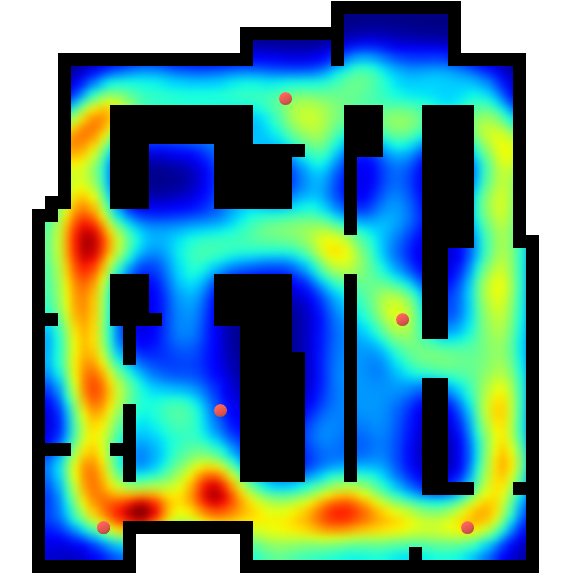
\includegraphics[width=\linewidth]{heat_corridors_safe}
     		\caption{Map ``Corridors'' with heuristic placement.}
     		\label{img:heat_corridors_safe}
 	\end{subfigure}
 	\hfill
  	\begin{subfigure}[t]{0.385\linewidth}
    		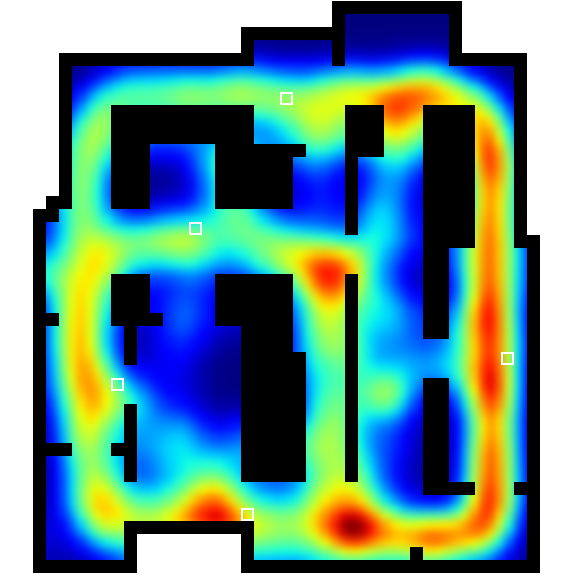
\includegraphics[width=\linewidth]{heat_corridors_uniform}
     		\caption{Map ``Corridors'' with uniform placement.}
     		\label{img:heat_corridors_uniform}
  	\end{subfigure}
 	\hfill
 	
 	\hfill
  	\begin{subfigure}[t]{0.385\linewidth}
		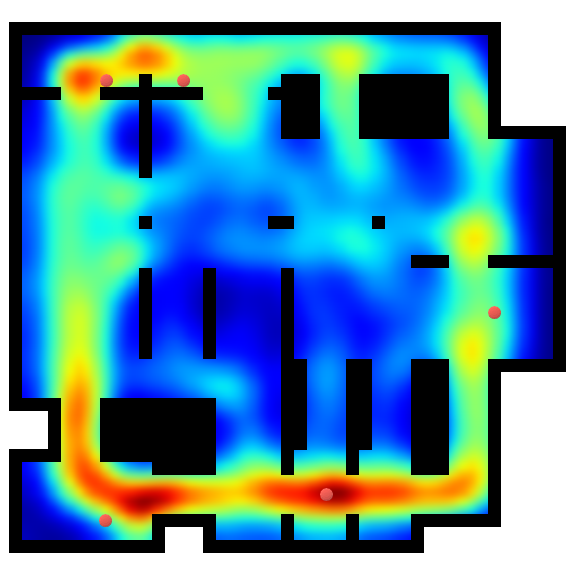
\includegraphics[width=\linewidth]{heat_intense_heuristic}
     		\caption{Map ``Intense'' with heuristic placement.}
     		\label{img:heat_intense_heuristic}
 	\end{subfigure}
 	\hfill
  	\begin{subfigure}[t]{0.385\linewidth}
    		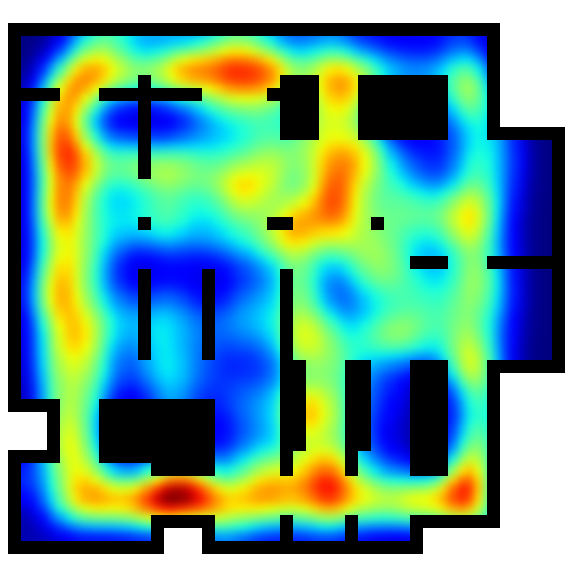
\includegraphics[width=\linewidth]{heat_intense_uniform}
     		\caption{Map ``Intense'' with uniform placement.}
     		\label{img:heat_intense_uniform}
  	\end{subfigure}	
  	\hfill
	\caption[Heat maps of the player position for the three maps used in the experiment.]{Heat maps of the player positions for the three maps used in the experiment. The red circles represent spawn points.}
	\label{img:heat}
\end{figure}

The position of spawn points also influenced the way in which users moved across the maps. Figure \ref{img:heat} shows, for each map and for each placement method, the heat maps of the sections that where crossed more frequently by the users. It is possible to notice that users, once understood the topology of the map, started to follow well defined \<farming routes>\footnote{In video games, \<farming routes> are regular closed paths defined to maximize the collection of certain resources in a specific map.}. These routes tend to be circular and to skirt the perimeter of the maps, with deviations that are influenced by the position of spawn points. The overall circularity is remarked by the heat maps associated to the uniform positioning, that being obtained by a set of five different uniform placements\footnote{The uniform \<study> has five \<cases>, whereas the heuristic \<study> has just one.}, represent an average route with respect to the possible position of spawn points.

\begin{figure}
\centering
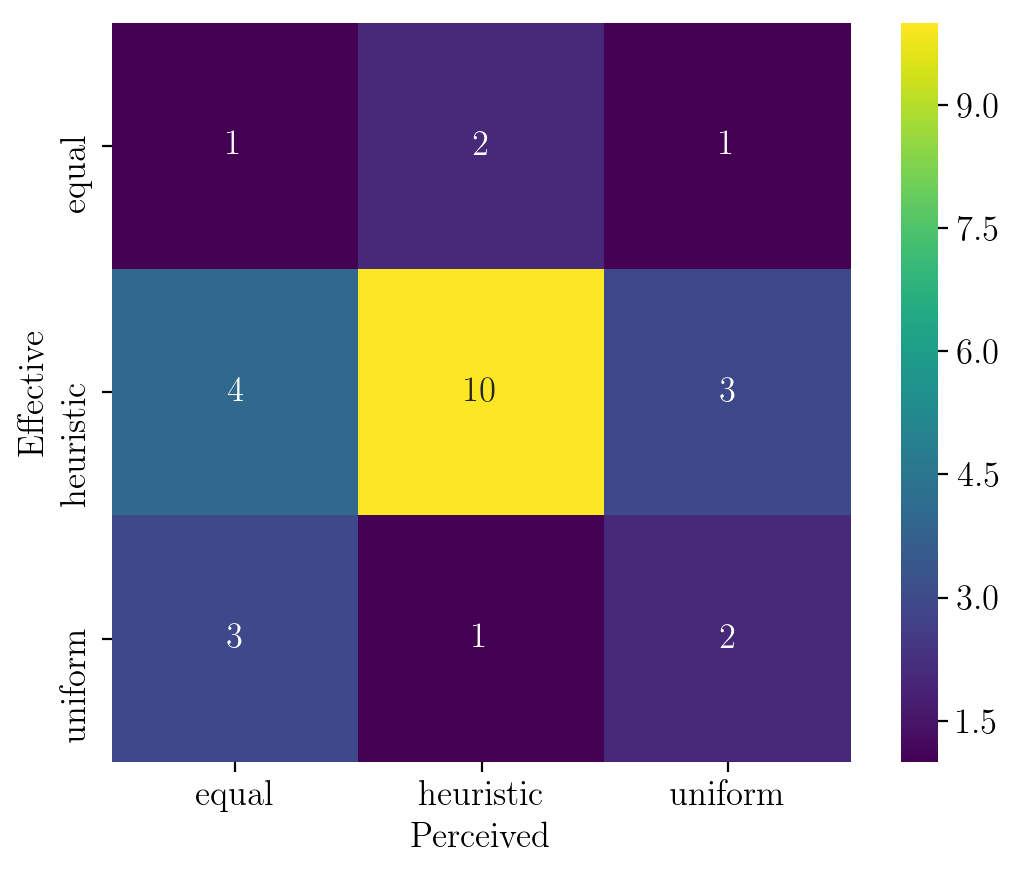
\includegraphics[width=0.8\linewidth]{difficulty}
\caption[Comparison between the effective and the perceived difficulty.]{Comparison between the effective and the perceived difficulty. Each square contains the number of samples where the user performed worst in the match with placement \<Effective> and evaluated as more difficult the match with placement \<Percived>. The match where a user performed worst is the one with the highest \<AvgKillTime>.}
\label{img:percived} 
\end{figure}

It is also interesting to notice how the difficulty in finding the targets was perceived by the users. As it can be seen in figure \ref{img:percived}, in the survey the majority of the users classified as more difficult the match where they performed worst, but some of them answered with the one where they performed better. 

\par

Finally, the intuition of flipping one of the two maps was correct, since many users believed to have played two completely different maps. 

% SUMMARY %

\section{Summary}

In this chapter we analyzed the experiment that we setup and its results, that proved the effectiveness of our heuristics and of our framework. We observed that the heuristic placement makes the targets harder to find, whereas the total distance covered by the user and the shooting accuracy are not influenced by the employed placement method. We also discovered that our heuristics work better with maps that do not have an uniform topology and we observed that users tend to define and follow specific routes when performing a research.